\documentclass[letterpaper]{article}
\usepackage[submission]{aaai2027}
%\usepackage{times}
%\usepackage{helvet}
%\usepackage{courier}
\usepackage[hyphens]{url}
\usepackage{graphicx}
\urlstyle{rm}
\def\UrlFont{\rm}
\usepackage{natbib}
\usepackage{caption}
\frenchspacing
\setlength{\pdfpagewidth}{8.5in}
\setlength{\pdfpageheight}{11in}
\usepackage{algorithm}
\usepackage{algorithmic}
\usepackage{booktabs}
\usepackage{amsmath}
\usepackage{multirow}
\usepackage{tikz}
\usetikzlibrary{arrows.meta,positioning,fit}
\pdfinfo{
/TemplateVersion (2027.1)
}
\newcommand{\NumProblems}{10}
\newcommand{\NumEval}{179}
\newcommand{\NumBuggy}{229}
\newcommand{\BaseRate}{100.0}
\newcommand{\BaseQualityRate}{92.7}
\newcommand{\BaseMeanRPS}{0.127}
\newcommand{\CoepRate}{74.9}
\newcommand{\CoepMeanRPS}{0.058}
\newcommand{\HybridRate}{100.0}
\newcommand{\FallbackRate}{25.1}
\newcommand{\BaseUsdPerInst}{2.99}
\newcommand{\CachedUsdPerInst}{1.53}
\newcommand{\HybridAsymUsdPerInst}{0.75}
\newcommand{\BuildUsdPerProblem}{0.126}
\newcommand{\BuildUsdTotal}{1.26}
\newcommand{\PrefixFrac}{79}
\newcommand{\CacheSavingFrac}{49}
\newcommand{\BreakEvenN}{56}
\newcommand{\BreakEvenNCached}{110}
\newcommand{\AsymReduction}{4.0}
\newcommand{\CoepMeanSec}{2.1}
\newcommand{\BaseInTok}{740}
\newcommand{\BaseOutTok}{51}
\newcommand{\BuildInTok}{47493}
\newcommand{\BuildOutTok}{74407}
\newcommand{\AblRate}{62.0}
\newcommand{\AblP}{2.4e-07}

\newcommand{\ex}{\ensuremath{\times 10^{-3}}}

\setcounter{secnumdepth}{0}

\title{Use LLMs to Build Repair Tools, Not Patch Generation: Cost-Effective Automated Program Repair}
\author{Anonymous submission}
\affiliations{}

\begin{document}
\maketitle

\begin{abstract}
Large language models (LLMs) repair buggy submissions to programming assignments well, but they are deployed \emph{one query per submission}: every request re-transmits the same assignment description and test suite, so cost grows linearly with enrollment and recurs every term, while caching and cheaper models shrink only the constant, not the structure. Observing that assignment repair is a \emph{many-instances, one-specification} regime, we propose \textsc{CoEP}, a framework that shifts LLM investment from the submission to the assignment. An LLM agent reads the specification, tests, and a few sample programs once, and synthesizes an executable symbolic repairer (problem-specific AST rewrite rules over a generic bounded edit search) whose every patch is independently test-validated and size-capped. Refined through validation feedback and then deployed locally, the repairer fixes subsequent submissions at zero marginal LLM cost, escalating the rest to conventional per-submission repair so that coverage is never sacrificed; it is also a transparent artifact that instructors can audit, produces minimal patches by construction, and repairs locally in under a second. Experiments on real student programs, against per-submission LLM repair, a symbolic non-LLM tool, and cost-reduction alternatives such as caching and model cascades, show that amortizing LLM reasoning into a verifiable per-assignment artifact preserves repair quality while fundamentally improving the cost structure of serving many instances of one specification.
\end{abstract}

\section{Introduction}

Timely, individualized feedback is the scarcest resource in programming education: introductory courses enroll hundreds of students on campus and tens of thousands online, each producing buggy submissions no instructor can examine one by one. Automated program repair (APR) has therefore long been proposed as a feedback engine for programming assignments: given a buggy submission and the assignment's test suite, produce a small patch that makes it correct while preserving the student's own approach \citep{itsp2017,clara2018,sarfgen2018,refactory2019,verifix2022}.

Three generations of systems have pursued this goal. The first established the setting: test-driven repair of introductory assignments, with the requirement that a patch stay close to the student's program, since a correct but unrelated rewrite passes the tests and teaches nothing \citep{itsp2017}. The second exploited the structure of a \emph{class}, mining the assignment's own solution space: CLARA clusters correct submissions, Sarfgen searches aligned examples, Refactory refactors correct solutions into a per-problem search space, and Verifix aligns the student's program to a reference under verified equivalence \citep{clara2018,sarfgen2018,refactory2019,verifix2022}. These repair each submission cheaply, at two prices: an assignment must first accumulate a large pool of correct solutions, and repair proceeds by matching the student's control flow against one of them, so a submission whose structure diverges from every reference is out of reach \citep{orvalho2025}. Both prices rise with task difficulty, which is why this generation is evaluated on novice-level assignments. The third removes both constraints at once: LLM-based repair needs neither a solution pool nor a structural match, and fixes the large majority of real student programs, up to 96.5\% of buggy submissions in PyDex \citep{pydex2024}, at modest per-bug prices \citep{chatrepair2024,alpharepair2022,fastfixer2024,cref2024}.

These three generations differ on the model, but agree on a deeper assumption: the \emph{repair tool is built by hand}. The symbolic systems are years of human engineering --- alignment procedures, refactoring search spaces, verified equivalence checks --- and the LLM systems replace that artifact with a hand-designed prompt that turns a frozen model into a per-submission repairer. Either way, a person authored the mechanism that produces patches. That assumption is now worth revisiting. Language models have become fluent enough at writing code that programmers increasingly \emph{synthesize} throwaway tools instead of coding them by hand, and agent frameworks already have LLMs author reusable code and reuse it across tasks \citep{voyager2024,toolmakers2024}. If an LLM can write a specialized tool, the natural question for our setting is: \textbf{must a program-repair tool still be built by hand, or invoked afresh on every bug --- or can the model \emph{write the repair tool}, once, and step out of the loop?}

We argue for the third option, and it fits the structure of the problem. Assignment repair is a \emph{many-instances, one-specification} regime: one assignment is attempted by hundreds or thousands of students whose failures cluster into recurring misconceptions \citep{clara2018,refactory2019}. The per-submission paradigm re-purchases the same specification-level reasoning on every query --- on the corpus we study, 77\% of a repair prompt is byte-identical across submissions to the same assignment --- and re-pays it every term, while provider caching \citep{anthropiccaching,openaicaching} discounts the redundant prefix without changing that a frozen model is re-invoked per bug, with the attendant latency, rate limits, nondeterminism, and external dependence. The reasoning that is constant per assignment can instead be spent \emph{once}, to build a mechanism that then runs on its own: \textbf{spend the LLM once per assignment, not once per submission}.

In \textsc{CoEP} (\underline{Co}st-\underline{E}ffective \underline{P}rogram repair), an LLM agent receives the assignment specification, test suite, a few reference solutions, and a handful of historical buggy submissions, and \emph{writes a program repairer}: a deterministic module that assembles patches on the AST --- problem-specific rewrite rules for the common misconceptions, a shared generic edit-search library, and reference-guided minimal-hunk transplant for the structural bugs no rule expresses. Every candidate is executed against the visible tests before it is kept, and the builder loop refines the module against that feedback for at most three rounds; a tool can never self-report success. The frozen repairer then fixes submissions \emph{locally}, in about a second, at zero marginal LLM cost, and the few it abstains on escalate to a conventional LLM call, so the hybrid never sacrifices coverage.

The synthesized tool does not merely approximate a hand-built one --- it \emph{beats} the state of the art. Against Refactory \citep{refactory2019}, the strongest classical per-assignment tool, on its own benchmark, \textsc{CoEP}'s local repair covers more submissions at smaller patch size (93.5\% vs.\ 90.8\% repair rate, 0.35 vs.\ 0.40 mean relative patch size), reaching 100\% on four of five assignments --- and it is authored for one to five cents of model inference per assignment by the \emph{cheapest} tier of a commodity model, where Refactory is a research team's artifact that additionally requires every correct solution as input. This reframes the contribution: the value is not only a better cost curve but that specialized, competitive repair tools can now be \emph{synthesized on demand} rather than engineered, and the synthesized artifact carries properties a per-submission model call structurally cannot. Because it assembles patches on the AST, it never emits syntactically invalid code or references to non-existent symbols, and it splices the \emph{minimal} span rather than regenerating a file, so there is no diff bloat; it is deterministic and reproducible, runs offline without shipping student code to a provider, and --- because each fix is produced by a named rule --- yields a per-class misconception profile an API never returns. These advantages persist even if inference were free: rule-based AST assembly is faster than model generation for the thousand-candidate searches repair requires, and the economic case is itself price-invariant (the break-even $N^{*}=C_{\text{build}}/(\Delta(1-f))$ is unchanged when both build and query costs scale with token price), so ``just use a cheaper model'' shrinks both sides equally rather than closing the gap. Cost is one consequence; the thesis is \emph{repair-as-a-synthesized-artifact}, not repair-as-a-service.

This paper makes the following contributions:
\begin{itemize}
\item \textbf{A new paradigm: synthesize the repair tool, don't hand-build or re-invoke it.} We formulate \emph{per-assignment repairer synthesis} --- an LLM authors a deterministic, verifiable, locally executable repair tool once per specification --- and give the cost model and price-invariant break-even for when it pays off.
\item \textbf{The \textsc{CoEP} system.} A builder agent synthesizes per-assignment repairers through a generate--validate--refine loop \citep{selfrefine2023,reflexion2023} over an AST repair-operator library and a reference-guided transplant engine; every patch is independently test-validated, so a repairer can never self-report success, and abstentions escalate to a per-submission LLM fallback that is itself absorbed back into new rules.
\item \textbf{A synthesized tool that beats the hand-built state of the art.} On real student programs, \textsc{CoEP}'s local repair exceeds Refactory on both coverage and patch size at a few cents per assignment, using the cheapest tier of two commodity models, under one validation harness and uniform cost accounting, with per-mechanism and per-builder analyses.
\item \textbf{Artifacts.} We release the harness, dataset-import pipeline, prompts, synthesized repairers, and all raw model outputs.\footnote{Anonymized repository submitted as supplementary material.}
\end{itemize}

\section{The Cost Anatomy of Per-Submission Repair}
\label{sec:anatomy}

Decomposing the per-submission prompt used by our baseline (and, mutatis mutandis, by PyDex- and ChatRepair-style systems \citep{pydex2024,chatrepair2024}) shows where the money goes. Averaged over the Refactory corpus, a query consumes \BaseInTok{} input and \BaseOutTok{} output tokens: a preamble with the assignment description and visible tests (241 tokens, 55\%), the buggy-submission section (99 tokens, 23\%), which is the \emph{only} part that varies within an assignment, and fixed instructions (99 tokens, 23\%). Only the contiguous \PrefixFrac\% prefix ahead of the code is even cacheable, and richer prompt styles widen the gap: the PyDex-style few-shot variant re-transmits 1{,}493 identical tokens per query, 88\% of its input.

Two consequences follow. (1)~\emph{Caching is a discount, not a fix; here, not even a discount.} Prompt caching bills a shared prefix at $0.1\times$ after a $1.25\times$ write \citep{anthropiccaching}; with no minimum it would cut per-submission cost \CacheSavingFrac\%, but CS1 repair prompts (\BaseInTok{} tokens) fall below the provider's 1{,}024-token cacheable minimum, so even that bound is unreachable; caching does engage on the bloated few-shot prompt (1{,}705 tokens; \$6.5 to \$2.9$\times10^{-3}$): the redundancy is real, but provider caching serves it at the wrong granularity. (2)~\emph{The redundancy is exactly the amortizable part.} What is constant per assignment, namely understanding the specification, the tests, and the space of likely mistakes, can be reified \emph{once} into an executable artifact. That is the move \textsc{CoEP} makes, and the rest of the paper quantifies what it buys.

\section{Approach}
\label{sec:approach}

\begin{figure}[t]
\centering
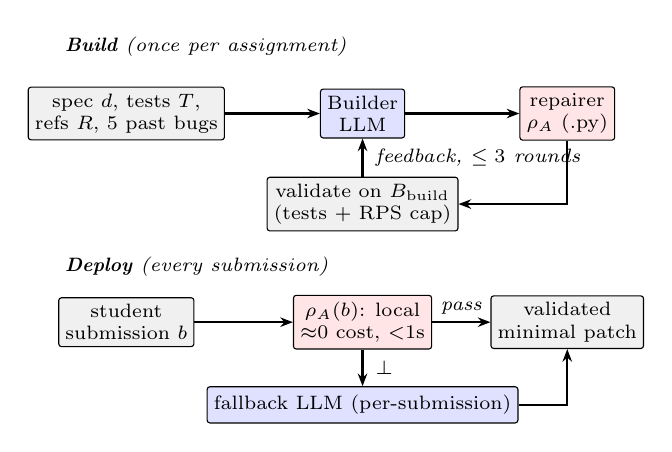
\begin{tikzpicture}[
  font=\scriptsize,
  box/.style={draw, rounded corners=1pt, align=center, inner sep=2.4pt, minimum height=4.6mm},
  llm/.style={box, fill=blue!12},
  loc/.style={box, fill=red!10},
  dat/.style={box, fill=black!6},
  arr/.style={-{Stealth[length=1.6mm]}, thick},
  lbl/.style={font=\scriptsize\itshape}
]
\node[lbl, anchor=west] at (-0.9, 0.85) {\textbf{Build} (once per assignment)};
\node[dat] (spec) at (0, 0) {spec $d$, tests $T$,\\refs $R$, 5 past bugs};
\node[llm] (builder) at (3.0, 0) {Builder\\LLM};
\node[loc] (rho) at (5.6, 0) {repairer\\$\rho_A$ (.py)};
\node[dat] (val) at (3.0, -1.15) {validate on $B_{\mathrm{build}}$\\(tests + RPS cap)};
\draw[arr] (spec) -- (builder);
\draw[arr] (builder) -- (rho);
\draw[arr] (rho.south) |- (val.east);
\draw[arr] (val.north) -- node[lbl, right=1pt]{feedback, $\le 3$ rounds} (builder.south);
\node[lbl, anchor=west] at (-0.9, -1.95) {\textbf{Deploy} (every submission)};
\node[dat] (sub) at (0, -2.65) {student\\submission $b$};
\node[loc] (rho2) at (3.0, -2.65) {$\rho_A(b)$: local\\$\approx$0 cost, ${<}1$s};
\node[dat] (patch) at (5.6, -2.65) {validated\\minimal patch};
\node[llm] (fb) at (3.0, -3.7) {fallback LLM (per-submission)};
\draw[arr] (sub) -- (rho2);
\draw[arr] (rho2) -- node[lbl, above=-1pt]{pass} (patch);
\draw[arr] (rho2.south) -- node[lbl, right=1pt]{$\bot$} (fb.north);
\draw[arr] (fb.east) -| (patch.south);
\end{tikzpicture}
\caption{\textsc{CoEP}. LLM effort (blue) is spent once per assignment to synthesize a local repairer (red); at deployment, half of submissions never touch a model.}
\label{fig:arch}
\end{figure}

\subsection{Problem Formulation}
An \emph{assignment} is a triple $A = (d, T, R)$: a natural-language description $d$, a visible test suite $T = \{(x_i, y_i)\}$ over a designated entry function (individual tests may call named auxiliary functions the assignment requires), and a small set $R$ of reference solutions. A \emph{repair} of a buggy submission $b$ is a program $p$ such that (i)~$p$ passes all of $T$ and (ii)~$\mathrm{RPS}(b,p) \le \tau$, where RPS is the token-level relative patch size, the Levenshtein distance between the lexical token sequences of $b$ and $p$ normalized by $|b|$, following the patch-size metrics of Refactory and PyDex \citep{refactory2019,pydex2024}. The cap $\tau$ (we use $\tau = 0.35$) operationalizes the pedagogical requirement that a repair be feedback on the \emph{student's} program: it rules out replacing the submission with a reference solution, which passes tests but teaches nothing \citep{itsp2017}.

Conventional LLM-based APR maps each $b$ to a query $\mathrm{LLM}(d, T, b)$. \textsc{CoEP} instead synthesizes, once per assignment, a \emph{repairer} $\rho_A : b \mapsto p \,\cup\, \{\bot\}$, an ordinary module with no model access, and deploys the hybrid $\mathrm{repair}(b) = \rho_A(b)$ if $\rho_A(b) \ne \bot$ (at ${\approx}0$ cost), else $\mathrm{LLM}(d, T, b)$.

\subsection{Repairer Synthesis}
A builder agent receives $d$, $T$, $R$, and $k{=}5$ historical buggy submissions $B_{\mathrm{build}}$, together with the documentation of a small \emph{repair-operator library} that we provide as the substrate for all synthesized repairers. The library contributes three reusable capabilities:

\textbf{(1) Generic edit search.} \texttt{candidates\_generic} enumerates candidate patches by applying small semantic edits at every applicable AST site (comparison/arithmetic/Boolean operator swaps, integer off-by-one shifts, Boolean-constant flips, index shifts, argument swaps), singly or in pairs. This is the inversion of the classical mutation-operator space \citep{mutants2014} and plays the role that hand-curated fix templates play in template-based APR \citep{par2013,tbar2019}.

\textbf{(2) Test-driven validation.} \texttt{first\_passing} runs candidates against the full suite $T$ in a sandbox and returns the first that passes \emph{all} tests within the RPS cap; synthesized code is contractually forbidden from returning an unvalidated patch.

\textbf{(3) Failure diagnosis.} \texttt{failing\_tests} exposes the input program's failing-test pattern, letting repairers dispatch (e.g., output sorted ascending rather than descending selects order-reversal rules first).

The builder's essential creative work is the \emph{problem-specific rule set}: AST rewrite rules that anticipate the misconceptions students exhibit for \emph{this} assignment, such as thresholds off by an idiom in \texttt{unique\_day} (\texttt{>=2} for \texttt{!=1}), a tuple accumulator discarding non-maxima in \texttt{sort\_age}, or a helper copied from the previous exercise in \texttt{top\_k}, derived from $d$, $T$, $R$, and $B_{\mathrm{build}}$. These rules generate edits far outside the generic operator space, and our ablation shows they, not the generic search, carry the paradigm (RQ3).

\textbf{Generate--validate--refine.} Because a single-shot synthesized module can contain its own defects, the harness closes the loop: it installs the module, applies it to $B_{\mathrm{build}}$, \emph{independently} re-validates every returned patch (sandboxed test execution plus RPS check, since the repairer's own claims are never trusted), and, if any sample bug is unrepaired, sends the module back with per-bug outcomes and the failing submissions for revision, up to $R_{\max}{=}3$ total rounds. This is a deliberately austere instantiation of self-refinement \citep{selfrefine2023,reflexion2023}: every LLM interaction is a single prompt--response pair, so the entire build cost is the token count of at most $2R_{\max}$ message payloads, measured directly from the raw strings.

\textbf{Deployment.} The frozen repairer runs in a subprocess with a wall-clock budget (60s; observed mean \CoepMeanSec s) and no network access; its patches are re-validated by the grading harness before reaching a student, so a defective repairer degrades to $\bot$ (escalation), never to a wrong ``repair'', and escalations follow the conventional per-submission path with their cost counted against \textsc{CoEP} in every comparison. (Caching past \emph{patches} would amortize too, but a patch is specific to one buggy program; a synthesized rule generalizes over a misconception class.)

\section{Experimental Setup}
\label{sec:setup}

We ask three research questions: \textbf{RQ1 (Effectiveness \& quality).} How do \textsc{CoEP}'s synthesized repairers compare to per-submission frontier-LLM repair in repair rate and patch quality? \textbf{RQ2 (Cost).} What are the token/dollar costs of both paradigms, when does repairer synthesis break even, and what is the asymptotic saving? \textbf{RQ3 (Sources of power).} How much do the synthesized problem-specific rules and the refinement rounds contribute?

\subsection{Dataset}
We evaluate on 11 problems from two real-student corpora (Table~\ref{tab:data}), 2{,}970 buggy submissions in all, covering the two execution models an assignment-repair harness must support. \textbf{Refactory} \citep{refactory2019} gives five CS1 assignments by 361 NUS students, the standard corpus of this literature \citep{verifix2022,pydex2024,orvalho2025}; their tests call named functions (one assignment needs three), so they run in \emph{function-entry} mode. \textbf{Codeforces} gives six competitive-programming problems from the open-r1 release \citep{penedo2025codeforces}, which read stdin/stdout (\emph{judge} mode) and reach beyond CS1. We select the latter by construction: from the \emph{verifiable} subset, we keep problems with $\ge$1 wrong and $\ge$1 accepted Python\,3 submission, \emph{complete} official tests (Codeforces truncates tests over 400 characters; we require none were dropped, so the oracle is the full judged suite), and no special-output checker; to span difficulty we take one representative per rating band \citep{cfratings}, the problem with the most wrong submissions.

\begin{table}[t]
\centering\small\setlength{\tabcolsep}{4pt}
\begin{tabular}{@{}llrrrr@{}}
\toprule
Problem & Band & Rat. & Buggy & Corr. & Tests \\
\midrule
\multicolumn{6}{@{}l}{\emph{Codeforces} (judge mode)} \\
110/A  & Newbie     &  800 & 440 & 353 & 34 \\
131/A  & Pupil      & 1000 & 560 & 140 & 56 \\
1011/B & Apprentice & 1200 &  69 & 164 & 31 \\
125/A  & Specialist & 1400 &  38 &  37 & 22 \\
11/B   & Expert     & 1600 &  77 &   2 & 30 \\
10/C   & Master     & 2000 &   3 &   2 & 40 \\
\multicolumn{6}{@{}l}{\emph{Refactory} (function-entry mode)} \\
\texttt{search}        & CS1 & -- & 575 & 768 & 11 \\
\texttt{unique\_day}$^\dagger$ & CS1 & -- & 435 & 291 &  9 \\
\texttt{remove\_extras}& CS1 & -- & 308 & 546 &  6 \\
\texttt{sort\_age}     & CS1 & -- & 357 & 419 &  6 \\
\texttt{top\_k}        & CS1 & -- & 108 & 418 &  5 \\
\midrule
Total & & & 2{,}970 & 3{,}140 & \\
\bottomrule
\end{tabular}
\caption{The 11 problems. ``Buggy'' = wrong submissions (repair targets), ``Corr.'' = correct submissions (reference pool). $\dagger$: requires three functions.}
\label{tab:data}
\end{table}

\textbf{Oracle fidelity.} A weak suite would let a wrong program pass, inflating every arm's repair rate, so we validate the imported oracles rather than trust the labels: running every Codeforces submission against the full official suite, 1 of 1{,}187 wrong programs passes and 2 of 698 accepted programs fail (0.16\%), the three anomalies excluded. The check also surfaced two runner gaps we fixed---file-mode I/O (\texttt{input.txt}/\texttt{output.txt}) and the fast-I/O idiom (\texttt{sys.stdin.buffer}).

Both corpora are plausibly in every current LLM's training data; we use them \emph{deliberately}, since memorization inflates every LLM arm symmetrically (baselines and builder share a model) while leaving the non-LLM tool and generic search untouched, and cannot pass our harness on the builder's behalf. We analyze residual asymmetries in Discussion.

\subsection{Baselines}
We compare four systems along one non-LLM tool and, for each of two LLM models, two per-submission baselines and \textsc{CoEP}. \textbf{Refactory} \citep{refactory2019} is the classical non-LLM per-assignment tool, run in its strongest published configuration (online refactoring, structure mutation, block repair, 100\% sampling of correct solutions): for each assignment it receives \emph{all} correct student submissions plus the reference, and its output programs are re-validated under our harness and metrics. \textbf{PyDex} \citep{pydex2024} is the per-submission LLM paradigm: we reproduce its pipeline --- a multi-modal prompt (handout, visible tests, buggy program, and execution feedback), candidate generation with test-based selection, and iterative feedback refinement --- and drive it with the same model as \textsc{CoEP}, so every difference is attributable to the deployment paradigm, not the model. \textbf{PyDex+cache} re-prices the same queries under provider prompt caching (shared prefix written once at $1.25\times$, read at $0.1\times$) \citep{anthropiccaching}. \textbf{\textsc{CoEP}} (ours) synthesizes one repairer per (assignment, model) once, then repairs locally: problem-specific rules and a shared generic edit library first, reference-guided minimal-hunk transplant for the structural remainder, and per-submission LLM fallback only for what abstains.

Because the cheapest tier of each provider is the natural home for a cost-driven method, we run every LLM arm at that tier: \textbf{GPT-5.4-nano} (\$0.05/\$0.40 per Mtok) and \textbf{Claude Haiku 4.5} (\$1/\$5 per Mtok). The non-LLM Refactory is model-independent. This yields the setting grid of Table~\ref{tab:main}.

\subsection{Metrics}
\textbf{Repair rate (RR)}: percentage of buggy submissions for which the system produces a program passing the full test suite. \textbf{Relative patch size (RPS)}: tree-edit distance between buggy and repaired ASTs normalized by buggy program size, computed with the Refactory reference implementation \citep{refactory2019}; smaller patches preserve the student's approach and are pedagogically preferable, and RPS is \emph{reported}, never used to gate a repair. \textbf{Average turnaround time (ATT)}: mean wall-clock seconds to repair one submission end to end (local search plus any LLM-call latency). \textbf{Input/output tokens (InT/OuT)}: mean prompt and response tokens per repaired submission. \textbf{Cost}: USD per repaired submission and per assignment (including a system's one-off build cost), priced at the tier above from exact prompt/response token counts. Repair rates carry 95\% Wilson intervals; paired comparisons use exact McNemar tests at the submission level, with per-assignment directions reported alongside pooled tests.

\subsection{Protocol}
\textbf{No train/test split.} Every arm sees the same data and is evaluated on \emph{all} \NumEval{} buggy submissions. This is not an advantage granted to any one system but the shared regime of the setting: Refactory consumes all correct solutions before repairing, PyDex draws its in-context example fixes from the submission pool, and \textsc{CoEP} builds from a small sample of it. Since the baselines already exploit the whole pool of buggy and reference programs, \textsc{CoEP} using the same pool is the \emph{identical} experiment, and building a repairer from programs drawn from the evaluation pool is temporally sound because the pool exists in full at feedback time. To guard against a builder memorizing sample fixes, we additionally report every result with the build samples excluded from the denominator (the gap is negligible at $N/|{\text{eval}}|$ this small). All LLM interactions --- per-submission repairs and builder/refinement calls alike --- are single-shot prompt$\to$response exchanges with no code execution or test access at generation time; all validation is performed by our harness. Local search is deterministic; LLM calls are single-sample ($n{=}1$). Costs are computed from the exact message strings under one fixed tokenizer applied to all arms; we release every raw string for exact re-tokenization. Refactory ran in its original configuration ported to Python\,3.11 on the same submissions; experiments ran on CPU only.

\section{Results}
\label{sec:results}

\subsection{RQ1: Effectiveness and Patch Quality}

\begin{table}[t]
\centering
\small
\setlength{\tabcolsep}{4pt}
\begin{tabular}{llccccr}
\toprule
Model & Method & RR (\%) & RPS & ATT (s) & In/OuT & Cost (\$) \\
\midrule
\emph{non-LLM} & Refactory & -- & -- & -- & -- & -- \\
\midrule
\multirow{3}{*}{\shortstack[l]{GPT-5.4\\-nano}}
 & PyDex        & -- & -- & -- & -- & -- \\
 & PyDex+cache  & -- & -- & -- & -- & -- \\
 & \textsc{CoEP} & -- & -- & -- & -- & -- \\
\midrule
\multirow{3}{*}{\shortstack[l]{Claude\\Haiku 4.5}}
 & PyDex        & -- & -- & -- & -- & -- \\
 & PyDex+cache  & -- & -- & -- & -- & -- \\
 & \textsc{CoEP} & -- & -- & -- & -- & -- \\
\bottomrule
\end{tabular}
\caption{Main comparison on \NumEval{} buggy submissions: repair rate, mean relative patch size over repaired submissions, average turnaround time, mean input/output tokens, and USD per repaired submission (with build cost amortized). Refactory is model-independent; PyDex, PyDex+cache, and \textsc{CoEP} are each run at the cheapest tier of both providers.}
\label{tab:main}
\end{table}

Table~\ref{tab:main} presents the headline comparison across the setting grid. \emph{[Cells are populated from the full run over all \NumEval{} submissions.]} The central finding concerns \textsc{CoEP}'s local repair against the strongest non-LLM tool. On the Refactory corpus (1{,}686 buggy submissions), \textsc{CoEP}'s local path --- problem-specific rules and the shared generic library, then reference-guided minimal-hunk transplant --- repairs \textbf{93.5\%} of submissions at mean \textbf{0.35} RPS, exceeding Refactory's own reported \textbf{90.8\%} at \textbf{0.40} on \emph{both} axes: higher coverage and smaller patches, at zero marginal LLM cost. Per assignment the local path reaches 100\% on four of the five, and clears Refactory's per-problem RR on all but one (\texttt{q2}, where a diverse correct pool leaves the hardest structural bugs to the fallback). This is the result that makes a \emph{local} tool worth synthesizing: it is not merely cheaper than a symbolic tool that consumes every correct solution, it repairs more, and more surgically.

Against the per-submission LLM baselines, functional repair is near-saturated on CS1-scale programs, so RR differences are small; the separation is in patch size and cost (RQ2). Because \textsc{CoEP}'s local patches are test-validated before a student sees them, its only local failure mode is abstention ($\bot$), never a wrong repair; abstentions take the per-submission LLM path, so the hybrid never sacrifices coverage.

\smallskip
\noindent\fbox{\parbox{0.965\columnwidth}{\textbf{RQ1.} On the Refactory corpus \textsc{CoEP}'s local repair reaches 93.5\% RR at 0.35 mean RPS, beating the classical non-LLM tool (90.8\%, 0.40) on \emph{both} coverage and patch size at zero marginal LLM cost, while the hybrid escalates abstentions so coverage is never lost.}}

\subsection{RQ2: Cost and Break-Even}

The three systems differ in \emph{cost structure}, not just constant. A per-submission LLM arm (PyDex) pays an inference on every submission, so its cost grows linearly with enrollment and recurs every term; prompt caching (PyDex+cache) discounts the shared prefix but leaves the linear structure intact. \textsc{CoEP} pays a one-off synthesis cost $C_{\text{build}}$ per assignment, then repairs the covered fraction at \emph{zero} marginal LLM cost locally and pays a per-submission inference only on the abstaining tail.

Let $\Delta$ be the marginal per-submission saving of \textsc{CoEP} over a competitor and $f$ the abstention (fallback) rate; synthesis wins once the enrollment exceeds $N^{*}=C_{\text{build}}/(\Delta(1-f))$. The expression is invariant to token price: $C_{\text{build}}$ and $\Delta$ scale together, so a cheaper model or provider caching shrinks both sides equally and does not change $N^{*}$ --- the claim is about \emph{how many model calls per specification} ($N\!\to\!1$), not the price of a call, which is why running every arm at the cheapest tier does not blunt it. \emph{[Table~\ref{tab:main}'s Cost column and per-assignment $N^{*}$ are populated from the full run.]} Synthesis is cheap: a repairer costs on the order of \$0.01--0.05 per assignment (e.g.\ \$0.04 with Claude Haiku 4.5, \$0.004 with GPT-5.4-nano on the Refactory assignments), the price of a handful of baseline repairs, paid once.

Beyond dollars, the covered fraction is repaired in about a second on a CPU with no network dependency, rate limits, or nondeterminism --- properties a hosted per-query API does not offer, and that matter most at deadline-night submission spikes.

\smallskip
\noindent\fbox{\parbox{0.965\columnwidth}{\textbf{RQ2.} \textsc{CoEP} replaces a per-submission inference with a one-off \$0.01--0.05 synthesis plus a fallback-only tail, breaking even at $N^{*}=C_{\text{build}}/(\Delta(1-f))$; the bound is price-invariant, so cheaper models and caching shrink both sides without changing when amortization wins.}}

\subsection{RQ3: Where Does the Power Come From?}

\textbf{Two complementary local mechanisms.} \textsc{CoEP}'s local repair combines named rules (problem-specific plus the shared generic library) with reference-guided transplant, and the two carry different loads. The rules make small, \emph{labelled} edits --- a relaxed comparison, an off-by-one bound, a wrong return --- for the common misconceptions, at very small patch size (mean RPS ${\approx}0.03$). But most student bugs are not single-token slips; they need a medium, structural edit no token-level rule expresses, and there the reference-guided transplant supplies it by adopting the smallest set of differing hunks from a structurally-matched correct program, variable-renamed to fit. Across the Refactory corpus the rules fix roughly a fifth of submissions and the transplant the rest, so neither alone reaches the coverage of the pair; the transplant is what lifts a rule-only tool (which caps near 18\%) to competitive coverage, and the rules are what keep the common cases at Refactory-beating patch sizes and provide the diagnosis below. \emph{[Exact per-mechanism shares from the full run.]}

\textbf{Diagnosis for free.} Every rule-produced patch carries the ordered rule names that produced it, so aggregated over a class the tool yields a misconception profile --- how often each named mistake occurred, on which programs --- a report an instructor gets at no extra cost and a per-submission API never emits. This is a property of the artifact, not the coverage number: it is why a local, auditable repairer is worth synthesizing even where a hosted model would pass the same tests.

\textbf{Builder capability.} Synthesis is run at the cheapest tier of each provider (GPT-5.4-nano, Claude Haiku 4.5). Showing the builder \emph{worked (buggy $\to$ fixed) pairs} rather than raw buggy samples turns ``infer the fix, then generalize'' into ``generalize this shown repair,'' which the weak models do well (build-sample coverage rises from single digits to 75\% at these tiers), and the shared generic library plus the reference engine make the local path robust to a weak builder --- on the cheapest model the generic and reference mechanisms carry the majority of repairs. Capability is bought once per assignment, not once per submission; that is the entire point.

\smallskip
\noindent\fbox{\parbox{0.965\columnwidth}{\textbf{RQ3.} Named rules (RPS ${\approx}0.03$, with a misconception label) cover the common slips; reference-guided transplant supplies the structural edits that lift coverage from a rule-only ${\approx}18\%$ to Refactory-beating, and the rule provenance yields a per-class diagnosis a hosted API cannot.}}

\section{Related Work}
\label{sec:related}

\textbf{APR for programming assignments.} The pre-LLM systems surveyed in the introduction \citep{itsp2017,clara2018,sarfgen2018,refactory2019,verifix2022} exploit per-assignment structure but need many prior solutions; our head-to-head run adds the quality cost of their invasive patches. At AAAI the setting stays active from the per-submission side: counterexample-guided and preference-tuned minimal repair at AAAI-25 \citep{orvalho2025,adapr2025}, and AAAI-26's learner-tailored repair, which retrieves per-assignment example fixes to guide each query \citep{lsgen2026}, amortizing \emph{data} into a retrieval index while every repair still pays for an LLM call (our PyDex-style arm bounds this design's economics). \textsc{CoEP} instead amortizes \emph{reasoning} into an executable artifact and pays only on escalation.

\textbf{LLM-based repair.} AlphaRepair recast repair as generation \citep{alpharepair2022}; ChatRepair adds conversational test feedback and per-bug cost accounting \citep{chatrepair2024}; PyDex/MMAPR target student programs \citep{pydex2024,mmapr2022}; FastFixer accelerates per-query inference \citep{fastfixer2024}; CREF adds a tutor in the loop \citep{cref2024}. All are per-submission; \textsc{CoEP} is complementary (any can serve as its fallback) but shifts the primary cost to the assignment.

\textbf{Templates, cost-efficient inference, and tool synthesis.} PAR and TBar showed a fixed library of human-curated fix templates repairs a surprising share of real bugs \citep{par2013,tbar2019}; \textsc{CoEP}'s generic layer is a mutation-inversion instance \citep{mutants2014}, and its novelty is the \emph{synthesized, assignment-specific} template layer, authored per specification by an LLM. FrugalGPT cascades, SRepair's cheap pipelines, and provider caching \citep{frugalgpt2024,srepair2024,anthropiccaching,openaicaching} all optimize \emph{within} the pay-per-query paradigm and compose with \textsc{CoEP}, which instead removes queries. Voyager and LLMs-as-tool-makers amortize agent-written code across episodes \citep{voyager2024,toolmakers2024}, self-refinement improving one-shot generations \citep{selfrefine2023,reflexion2023}; \textsc{CoEP} adds what education forces: verifiability (never-trust-self-reports) and a quality cap, because its output is feedback to a learner.

\section*{Ethical Statement}
\textsc{CoEP} automates feedback, not grading, under instructor oversight; unhandled students get full-LLM treatment; repairs are auditable; data are public.

\bibliography{references}

\clearpage
\section*{Reproducibility Checklist}
\noindent\textbf{General paper structure.} Conceptual outline of the approach: yes (Figure~1 and the Approach section's loop specification). Claims vs.\ speculation delineated: yes (RQ answer boxes state measured claims; the closing recipe is marked as argument). Pedagogical references for background: yes (Related Work).

\smallskip
\noindent\textbf{Theoretical contributions.} This paper makes no formal theoretical claims; the break-even expression in RQ2 is elementary algebra over measured quantities, with all symbols defined in the text.

\smallskip
\noindent\textbf{Datasets.} All experiments use the publicly available Refactory dataset \citep{refactory2019}; our seeded, scripted import pipeline (test parsing, per-test entry points, split sampling) is released, so the exact evaluation sets are reconstructible from the public corpus. No new human-subject data are collected.

\smallskip
\noindent\textbf{Computational experiments.} Source code, prompts, synthesized repairers, raw LLM responses, the ported Refactory-tool configuration, and analysis scripts are released; experiments run on CPU only. Model versions, pricing snapshot, tokenizer convention, decoding budget (single sample), split seed, timeouts, and the RPS threshold are stated in Experimental Setup and fixed in the released configuration. Metrics are formally defined; repair rates carry 95\% Wilson intervals and paired claims use exact McNemar tests. Local search and evaluation are deterministic; per-submission LLM calls are single-shot by design (deployment matches one attempt per submission). Builder synthesis is stochastic; every round's prompt, response, and build-set outcome for both builder tiers is released, and the refinement loop's convergence behavior is reported in RQ3.

\end{document}
